% -------------------- Acknowledgement -------------------------
%
% This latex file is copied from that prepared by Matthew Pitkin
% for his JOSS article:
%     psrqpy: a python interface for querying the ATNF pulsar catalogue
%     https://joss.theoj.org/papers/10.21105/joss.00538
%     https://arxiv.org/abs/1806.07809
%
% With modifications to the bibtex, hypersetup
% --------------------------------------------------------------
\documentclass[10pt,a4paper,onecolumn]{article}
\usepackage{marginnote}
\usepackage{graphicx}
\usepackage{xcolor}
\usepackage{authblk,etoolbox}
\usepackage{titlesec}
\usepackage{calc}
\usepackage{tikz}
\usepackage{hyperref}
\hypersetup{
    colorlinks=true,     % false: boxed links; true: colored links
    linkcolor=blue,      % color of internal links
    citecolor=blue,      % color of links to bibliography
    filecolor=blue,      % color of file links
    urlcolor=blue        % color of external links
}
\usepackage{caption}
\usepackage{tcolorbox}
\usepackage{amssymb,amsmath}
\usepackage{ifxetex,ifluatex}
\usepackage{seqsplit}
%\usepackage{fixltx2e} % provides \textsubscript
%\usepackage[
%  backend=bibtex,
%  style=alphabetic,
%  citestyle=numeric
%]{biblatex}
%\bibliography{paper.bib}


% --- Page layout -------------------------------------------------------------
\usepackage[top=3.5cm, bottom=3cm, right=1.5cm, left=1.5cm,
            headheight=2.2cm, reversemp, includemp, marginparwidth=4.0cm]{geometry}

% --- Default font ------------------------------------------------------------
% \renewcommand\familydefault{\sfdefault}

% --- Style -------------------------------------------------------------------
%\renewcommand{\bibfont}{\small \sffamily}
\renewcommand{\captionfont}{\small\sffamily}
\renewcommand{\captionlabelfont}{\bfseries}

% --- Section/SubSection/SubSubSection ----------------------------------------
\titleformat{\section}
  {\normalfont\sffamily\Large\bfseries}
  {}{0pt}{}
\titleformat{\subsection}
  {\normalfont\sffamily\large\bfseries}
  {}{0pt}{}
\titleformat{\subsubsection}
  {\normalfont\sffamily\bfseries}
  {}{0pt}{}
\titleformat*{\paragraph}
  {\sffamily\normalsize}


% --- Header / Footer ---------------------------------------------------------
\usepackage{fancyhdr}
\pagestyle{fancy}
\fancyhf{}
%\renewcommand{\headrulewidth}{0.50pt}
\renewcommand{\headrulewidth}{0pt}
\fancyhead[L]{\hspace{-0.75cm}
\includegraphics[width=5.5cm]{joss-logo.png}}
\fancyhead[C]{}
\fancyhead[R]{}
%\renewcommand{\footrulewidth}{0.25pt}



\fancyfoot[R]{\sffamily \thepage}
\makeatletter
\let\ps@plain\ps@fancy
\fancyheadoffset[L]{4.5cm}
\fancyfootoffset[L]{4.5cm}

% --- Macros ---------

\definecolor{linky}{rgb}{0.0, 0.5, 1.0}

\newtcolorbox{repobox}
   {colback=red, colframe=red!75!black,
     boxrule=0.5pt, arc=2pt, left=6pt, right=6pt, top=3pt, bottom=3pt}

\newcommand{\ExternalLink}{%
   \tikz[x=1.2ex, y=1.2ex, baseline=-0.05ex]{%
       \begin{scope}[x=1ex, y=1ex]
           \clip (-0.1,-0.1)
               --++ (-0, 1.2)
               --++ (0.6, 0)
               --++ (0, -0.6)
               --++ (0.6, 0)
               --++ (0, -1);
           \path[draw,
               line width = 0.5,
               rounded corners=0.5]
               (0,0) rectangle (1,1);
       \end{scope}
       \path[draw, line width = 0.5] (0.5, 0.5)
           -- (1, 1);
       \path[draw, line width = 0.5] (0.6, 1)
           -- (1, 1) -- (1, 0.6);
       }
   }

% --- Title / Authors ---------------------------------------------------------
% patch \maketitle so that it doesn't center
\patchcmd{\@maketitle}{center}{flushleft}{}{}
\patchcmd{\@maketitle}{center}{flushleft}{}{}
% patch \maketitle so that the font size for the title is normal
\patchcmd{\@maketitle}{\LARGE}{\LARGE\sffamily}{}{}
% patch the patch by authblk so that the author block is flush left
\def\maketitle{{%
  \renewenvironment{tabular}[2][]
    {\begin{flushleft}}
    {\end{flushleft}}
  \AB@maketitle}}
\makeatletter
%\renewcommand\AB@affilsepx{ \protect\Affilfont}
%\renewcommand\AB@affilnote[1]{{\bfseries #1}\hspace{2pt}}
\renewcommand\AB@affilnote[1]{{\bfseries #1}\hspace{3pt}}
\makeatother
\renewcommand\Authfont{\sffamily\bfseries}
\renewcommand\Affilfont{\sffamily\small\mdseries}
\setlength{\affilsep}{1em}


\ifnum 0\ifxetex 1\fi\ifluatex 1\fi=0 % if pdftex
  \usepackage[T1]{fontenc}
  \usepackage[utf8]{inputenc}

\else % if luatex or xelatex
  \ifxetex
    \usepackage{mathspec}
  \else
    \usepackage{fontspec}
  \fi
  \defaultfontfeatures{Ligatures=TeX,Scale=MatchLowercase}

\fi
% use upquote if available, for straight quotes in verbatim environments
\IfFileExists{upquote.sty}{\usepackage{upquote}}{}
% use microtype if available
\IfFileExists{microtype.sty}{%
\usepackage{microtype}
\UseMicrotypeSet[protrusion]{basicmath} % disable protrusion for tt fonts
}{}

%\usepackage{hyperref}
\hypersetup{unicode=true,
            pdftitle={EspressoDB: A scientific database for managing high-performance computing workflows.},
            pdfborder={0 0 0},
            breaklinks=true}
\urlstyle{same}  % don't use monospace font for urls
\usepackage{graphicx,grffile}
\makeatletter
\def\maxwidth{\ifdim\Gin@nat@width>\linewidth\linewidth\else\Gin@nat@width\fi}
\def\maxheight{\ifdim\Gin@nat@height>\textheight\textheight\else\Gin@nat@height\fi}
\makeatother
% Scale images if necessary, so that they will not overflow the page
% margins by default, and it is still possible to overwrite the defaults
% using explicit options in \includegraphics[width, height, ...]{}
\setkeys{Gin}{width=\maxwidth,height=\maxheight,keepaspectratio}
\IfFileExists{parskip.sty}{%
\usepackage{parskip}
}{% else
\setlength{\parindent}{0pt}
\setlength{\parskip}{6pt plus 2pt minus 1pt}
}
\setlength{\emergencystretch}{3em}  % prevent overfull lines
\providecommand{\tightlist}{%
  \setlength{\itemsep}{0pt}\setlength{\parskip}{0pt}}
\setcounter{secnumdepth}{0}
% Redefines (sub)paragraphs to behave more like sections
\ifx\paragraph\undefined\else
\let\oldparagraph\paragraph
\renewcommand{\paragraph}[1]{\oldparagraph{#1}\mbox{}}
\fi
\ifx\subparagraph\undefined\else
\let\oldsubparagraph\subparagraph
\renewcommand{\subparagraph}[1]{\oldsubparagraph{#1}\mbox{}}
\fi

\title{EspressoDB: A scientific database for managing high-performance computing workflow}

        \author[1,2,3]{Chia Cheng Chang}
        \author[2,3$\dagger$]{Christopher K{\"o}rber}
        \author[3,2]{Andr{\'e}~Walker-Loud}

      \affil[1]{iTHEMS RIKEN, Wako, Saitama 351-0198, Japan}
      \affil[2]{Department of Physics, University of California, Berkeley, California 94720, USA}
      \affil[3]{Nuclear Science Division, Lawrence Berkeley National Laboratory, Berkeley, California 94720}
      \affil[$\dagger$]{\textit {\href{mailto:software@ckoerber.com}{software@ckoerber.com}}}

  \date{\vspace{-5ex}}



\begin{document}
\maketitle

\marginpar{
  %\hrule
  \sffamily\small

  %{\bfseries DOI:} \href{XXX}{\color{linky}{TBD}}

  \vspace{2mm}

  {\bfseries Software}
  \begin{itemize}
    \setlength\itemsep{0em}
    \item \href{https://github.com/openjournals/joss-reviews/issues/1936}{\color{linky}{Review}} \ExternalLink
    \item \href{https://github.com/callat-qcd/espressodb}{\color{linky}{EspressoDB}} \ExternalLink
    \item \href{https://github.com/callat-qcd/lattedb}{\color{linky}{LattedDB}} \ExternalLink
  \end{itemize}



  \vspace{2mm}

  {\bfseries Submitted:} 06 Dec. 2019\\
  %{\bfseries Published:} XX XXX 20XX

  \vspace{2mm}
  {\bfseries Licence}\\
  Authors of papers retain copyright and release the work under a Creative Commons Attribution 4.0 International License (\href{http://creativecommons.org/licenses/by/4.0/}{\color{linky}{CC-BY}}).
}

%---------------------------------------------------------
% Main body
\hypertarget{summary}{%
\section{Summary}\label{summary}}

Leadership computing facilities around the world support cutting-edge
scientific research across a broad spectrum of disciplines including
understanding climate change \cite{Kurth\_2018}, combating opioid
addiction \cite{Joubert:2018:AOE:3291656.3291732}, or simulating the
decay of a neutron \cite{Berkowitz:2018gqe}. While the increase in
computational power has allowed scientists to better evaluate the
underlying model, the size of these computational projects have grown to
a point where a framework is desired to facilitate managing the
workflow. A typical scientific computing workflow includes:

\begin{enumerate}
\def\labelenumi{\arabic{enumi}.}
\tightlist
\item
  Defining all input parameters for every step of the computation;
\item
  Defining dependencies of computational tasks;
\item
  Storing some of the output data;
\item
  Post-processing these data files;
\item
  Performing data analysis on output.
\end{enumerate}

\href{https://github.com/callat-qcd/espressodb/}{\texttt{EspressoDB}} is
a programmatic object-relational data management framework implemented
in Python and based on the
\href{https://www.djangoproject.com}{\texttt{Django} web framework}.
\texttt{EspressoDB} was developed to streamline data management
workflows, centralize and guarantee data integrity, while providing
domain flexibility and ease of use.

The framework provided by \texttt{EspressoDB} aims to support the ever
increasing complexity of workflows of scientific computing at leadership
computing facilities (LCFs), with the goal of reducing the amount of
human time required to manage the jobs, thus giving scientists more time
to focus on science.

\hypertarget{features}{%
\section{Features}\label{features}}

Data integrity is important to scientific projects and becomes more
challenging the larger the project. In general, a \texttt{SQL} framework
type-checks data before writing to the database and controls
dependencies and relations between different tables to ensure internal
consistency. \texttt{EspressoDB} allows additional user-defined
constraints not supported by \texttt{SQL} (\emph{e.g.} unique
constraints using information across related tables). Once the user has
specified a set of conditions that entries have to fulfill for each
table, \texttt{EspressoDB} runs these cross checks for new data before
inserting them in the database.

\texttt{EspressoDB} also supports collaborative and open-data oriented
projects by leveraging and extending \texttt{Django}'s web hosting
component. In addition to providing a centralized data platform, it is
possible to spawn customized web pages which can be hosted locally or on
the world wide web\footnote{Depending on the configuration, it is
  possible to provide selected access for multiple users on different
  levels.}. \texttt{EspressoDB} simplifies creating projects by
providing default \texttt{Django} configurations that set up for
example, connections to the database and webpages to view associated
tables. For example, with the default setting, \texttt{EspressoDB}
spawns:

\begin{itemize}
\tightlist
\item
  Documentation views of implemented tables;
\item
  A project wide notification system;
\item
  Project specific Python interface guidelines which help writing
  scripts to populate the database;
\item
  Admin pages for interacting with data in a GUI.
\end{itemize}

Further views can be implemented to interact with data and use existing
Python libraries for summarizing and visualizing information. This
allows users to create visual progress updates on the fly and to
integrate the database information to the data-processing workflow,
significantly reducing the human overhead required due to improved
automation.

More details, usage instructions and examples are documented at
\href{https://espressodb.readthedocs.io}{espressodb.readthedocs.io}.

\hypertarget{use-case}{%
\section{Use case}\label{use-case}}

\href{https://github.com/callat-qcd/lattedb/}{\texttt{LatteDB}}, an
application of \texttt{EspressoDB} that is specialized to contain table
definitions for lattice quantum chromodynamics (LQCD) calculations and
analysis. \texttt{LatteDB} is currently being used by the
\href{https://a51.lbl.gov/~callat/webhome/}{CalLat Collaboration} in
their computations on Summit at the Oak Ridge Leadership Computing
Facility (\href{https://www.olcf.ornl.gov}{OLCF}) through DOE INCITE
Allocations \cite{incite:2019, incite:2020}. The website generated by
\texttt{LatteDB} used by CalLat can be found at
\url{https://ithems.lbl.gov/lattedb/}. A precursor to
\texttt{EspressoDB} and \texttt{LatteDB} was used to support a series of
LQCD projects \cite{Nicholson:2018mwc, Chang:2018uxx}.

Summit at OLCF is disruptively fast compared to previous generations of
leadership class computers. There are two challenges which are both
critical to address for near-exascale computers such as Summit, which
will become more important in the exascale era:

\begin{enumerate}
\def\labelenumi{\arabic{enumi}.}
\item
  \emph{Efficient bundling and management of independent tasks}: LCFs
  prohibit the submission of millions of small tasks to their
  supercomputers (clogged queues, overtaxed service nodes etc.). It is
  imperative to have a task manager capable of bundling many tasks into
  large jobs while distributing the work to various components of the
  heterogeneous nodes;
\item
  \emph{Dependent task generation and data processing}: As an example,
  CalLat creates peta-bytes of temporary files that are written to the
  scratch file system, used for subsequent computations and ultimately
  processed down to hundred of tera-bytes that are saved for analysis.
  It is essential to track the status of these files in real-time
  (identify corrupt, missing, or purgeable files).
\end{enumerate}

Members of CalLat are addressing issue 1 through the creation of job
management software,
\href{https://github.com/evanberkowitz/metaq}{METAQ}
\cite{Berkowitz:2017vcp} and \texttt{MPI\_JM} \cite{Berkowitz:2018gqe;
Berkowitz:2017xna}. \texttt{LatteDB} is designed to address the
second issue. A future feature of \texttt{LatteDB} is integration with
\texttt{MPI\_JM}.

\hypertarget{acknowledgements}{%
\section{Acknowledgements}\label{acknowledgements}}

We thank Even Berkowitz, Arjun Gambhir, Ben Hörz, Kenneth McElvain and
Enrico Rinaldi for useful insights and discussions which helped in
creating \texttt{EspressoDB} and \texttt{LatteDB}. C.K. gratefully
acknowledges funding through the Alexander von Humboldt Foundation
through a Feodor Lynen Research Fellowship. The work of A.W-L. was
supported by the Exascale Computing Project (17-SC-20-SC), a joint
project of the U.S. Department of Energy's Office of Science and
National Nuclear Security Administration, responsible for delivering a
capable exascale ecosystem, including software, applications, and
hardware technology, to support the nation's exascale computing
imperative.

This research used resources of the Oak Ridge Leadership Computing
Facility, which is a DOE Office of Science User Facility supported under
Contract DE-AC05-00OR22725, with access and computer time granted
through the DOE INCITE Program.

\hypertarget{references}{%
\section{References}\label{references}}


%---------------------------------------------------------
% bib file

\bibliography{paper}
\bibliographystyle{ieeetr}

\appendix
\section{Supplemental Information}

\subsection{Django overview\label{django-overview}}

\texttt{EspressoDB} utilizes Python's \texttt{Django} Object-Relational
Mapping (ORM) framework. Tables correspond to Python classes, rows
correspond to instances and columns correspond to attributes of the
instances.  One can filter instances by their attributes
or generate summary tables (\texttt{pandas.DataFrame}) within one line
of code. Furthermore, using an ORM allows one to have the same interface
independent of the backend. It is possible to store data in a file based
\texttt{SQLite} solution, or use more scalable options like
\texttt{MySQL} or \texttt{Postgresql}.

\texttt{Django} is part of many open-source projects and thus comes with
extensive documentation. Additionally, \texttt{Django} is scalable,
comes with reliable tests and vast community support which manifests in
the fact that it is commonly used in large scale projects (BitBucket,
Instagram, Mozilla, NASA and many more). One guiding principle of
\texttt{EspressoDB} is to not ``re-invent the wheel'' but instead
leverage the support coming from \texttt{Django}. As a result, one can
easily incorporate many of \texttt{Django}'s extensions and find
solutions to technical questions online.

\subsection{Lattice QCD use case \label{lattice-qcd-use-case}}

LQCD is an inherently a stochastic method of simulating quantum
chromodynamics (QCD) the fundamental theory of nuclear strong
interactions, which is responsible for confining quarks into protons and
neutrons and ultimately, for binding these nucleons into the atomic
nuclei we observe in nature. The application of LQCD to forefront
research applications in nuclear physics is necessary to build a
quantitative connection between our understanding of nuclei and QCD.
This is important as nuclei serve as laboratories and/or detectors for
many experiments aiming to test the limits of the Standard Model of
particle physics in our quest to understand questions such as: Why is
the universe composed of matter and not anti-matter? Does dark matter
interact with regular matter other than gravitationally? What is the
nature of the neutrino and is it related to the observed excess of
matter over anti-matter? See Ref. \cite{Drischler:2019xuo} for a recent
review of the interface of LQCD with our understanding of nuclear
physics.

The application of LQCD to nuclear physics is an exascale challenge. One
of the main reasons these calculations are so expensive is that when
LQCD is applied to systems of one or more nucleons, an exponentially bad
signal-to-noise problem must be overcome. While the optimal strategy for
overcoming this challenge is not yet known, one thing common to all
methods is the need for an exponentially large amount of statistics. As
such, these LQCD computations require the completion of millions of
independent sub-calculations (or tasks), with chained dependencies, in
order to complete a single calculation. These chained tasks write large
amounts of temporary files to the scratch file system which are used as
input for subsequent files, often with multiple input files required for
the later computations. Several such calculations must be performed in
order to extrapolate the results to the physical point, defined as the
limit of zero discretization (the continuum limit), the infinite volume
limit and the limit of physical quark masses which are \emph{a priori}
unknown and so must be determined through this
extrapolation/interpolation procedure. These requirements lead to a very
complex set of computations that must be carried out with great care and
a significant amount of human time and effort to ensure the computing
cycles are used as efficiently as possible.

Compounding these challenges, the new computer Summit, is
\emph{disruptively fast} compared to previous generations of leadership
class computers. Full machine-to-machine, Summit is approximately 15
times faster than Titan when applied to LQCD applications such as those
carried out by CalLat \cite{8665785}. While this is great for
scientific throughput, it also means the management of the computational
jobs has become unwieldy with the management models typically used for
such computations: Summit churns through the computations so fast, and
produces so much data, it is not possible to keep up with the data
processing and management with our older management tools.

As a concrete example, we consider the nucleon elastic form factor
project being carried out by CalLat \cite{incite:2019, incite:2020}.
For each \emph{ensemble} of gauge configurations used (one choice of
input parameters) the computation requires the following dependent
steps:

\begin{enumerate}
\def\labelenumi{\arabic{enumi}.}
\tightlist
\item
  For each gauge configuration (of O(1000)) in an ensemble (of O(20)),
  make several quark sources (grouped in batches of 8);
\item
  For each source, create a quark propagator;
\item
  For each quark propagator:

  \begin{enumerate}
  \def\labelenumii{\arabic{enumii}.}
  \tightlist
  \item
    Create a proton correlation function to determine the proton mass;
  \item
    Create O(10) proton \emph{sequential} sinks at different separation
    times (times 8 for different spin, flavor and parity combination);
  \end{enumerate}
\item
  For each time-separation, group the 8 \emph{sequential} sinks from the
  8 propagators into a single \emph{coherent sequential} sink
  \cite{Bratt:2010jn};
\item
  For each time-separation, Solve a \emph{sequential} propagator from
  the \emph{coherent sequential} sink;
\item
  For each time-separation, spin, flavor and parity, tie each of the original 8 propagators with
  the sequential propagator to construct a 4-dimensional (4D)
  \emph{formfactor} correlation function;
\item
  Process the data to prepare it for analysis and the extraction of
  physics.
\item
  Repeat for multiple source sets (of 8) if more statistics are
  required.
\end{enumerate}

Each of the steps above leads to the generation of many large
(multi-gigabyte) data files, most of which are not saved.
\texttt{LatteDB} is used to track the status of these data files to know
if they need to be created or if the next step can proceed. The final
data production step, 6, leads to our final data file that need further
processing prior to our final analysis and saving of the files.

Inheriting the functionality of \texttt{EspressoDB}, \texttt{LatteDB}
has the flexibility to faithfully reproduce a one-to-one mapping between
the above computational workflow to database tables. For example, in
step 1, the table of gauge configurations is defined such that every row
in the table specifies a single gauge configuration. This reflects how
on disk, we have thousands of files, each containing a snapshot of the
QCD vacuum, and as such, every file, and every subsequent file as a
result of the gauge configuration (\emph{e.g.} propagators or
correlation functions in steps 2 through 6) can also be tracked
individually. However, at the end of the calculation, an observable is
only well defined with an ensemble of gauge configurations.
\texttt{LatteDB} allows one to define an ensemble table, with a
\texttt{Django\ ManyToMany} data type which may be interpreted as a
single column containing a list of references (foreign keys) to the
table of gauge configurations. In \texttt{SQL}, a list of foreign keys
is not a fundamental data type that is supported, and is only made
possible with \texttt{Django}. However, even with \texttt{Django},
unique constraints can not be implemented on such a column. With
\texttt{LatteDB}, we make it possible to define a unique constraint,
which for this example, prohibits the user from inserting the exact same
list of gauge configurations in the ensemble table more than once. Users
are encouraged to consult the documentation of \texttt{EspressoDB} and
examples in \texttt{LatteDB} for more information.

Additionally, \texttt{LatteDB} is also tremendously useful for managing
the data processing steps (step 7) which proceed as:

\begin{enumerate}
\setcounter{enumi}{6}\item Data processing:
\begin{enumerate}
\item For each configuration, for each time separation, for each of the 8 sources, \emph{time slice} the 4D data \texttt{formfactor} files to only the time slices containing relevant data;

\item For each configuration, for each time separation, for each source set, average the 8 \texttt{formfactor\_tsliced} files to a source averaged file;

\item When all configurations are complete, concatenate these files together;

\item As needed, Fourier Transform these files to project the \texttt{formfactors} onto definite momentum transfers;

\item Analyze the correlation functions to extract the relevant physics.
\end{enumerate}
\end{enumerate}


In Figure 1, we show an example \texttt{LatteDB} Table from step 7b. The
user is able to filter on each column to very quickly assess the
production status (green means the \texttt{tsliced\_source\_averaged} file
exists, red means it is missing) and decide what configurations in what
ensembles need to be managed in production.

\begin{figure}[t!]
\centering
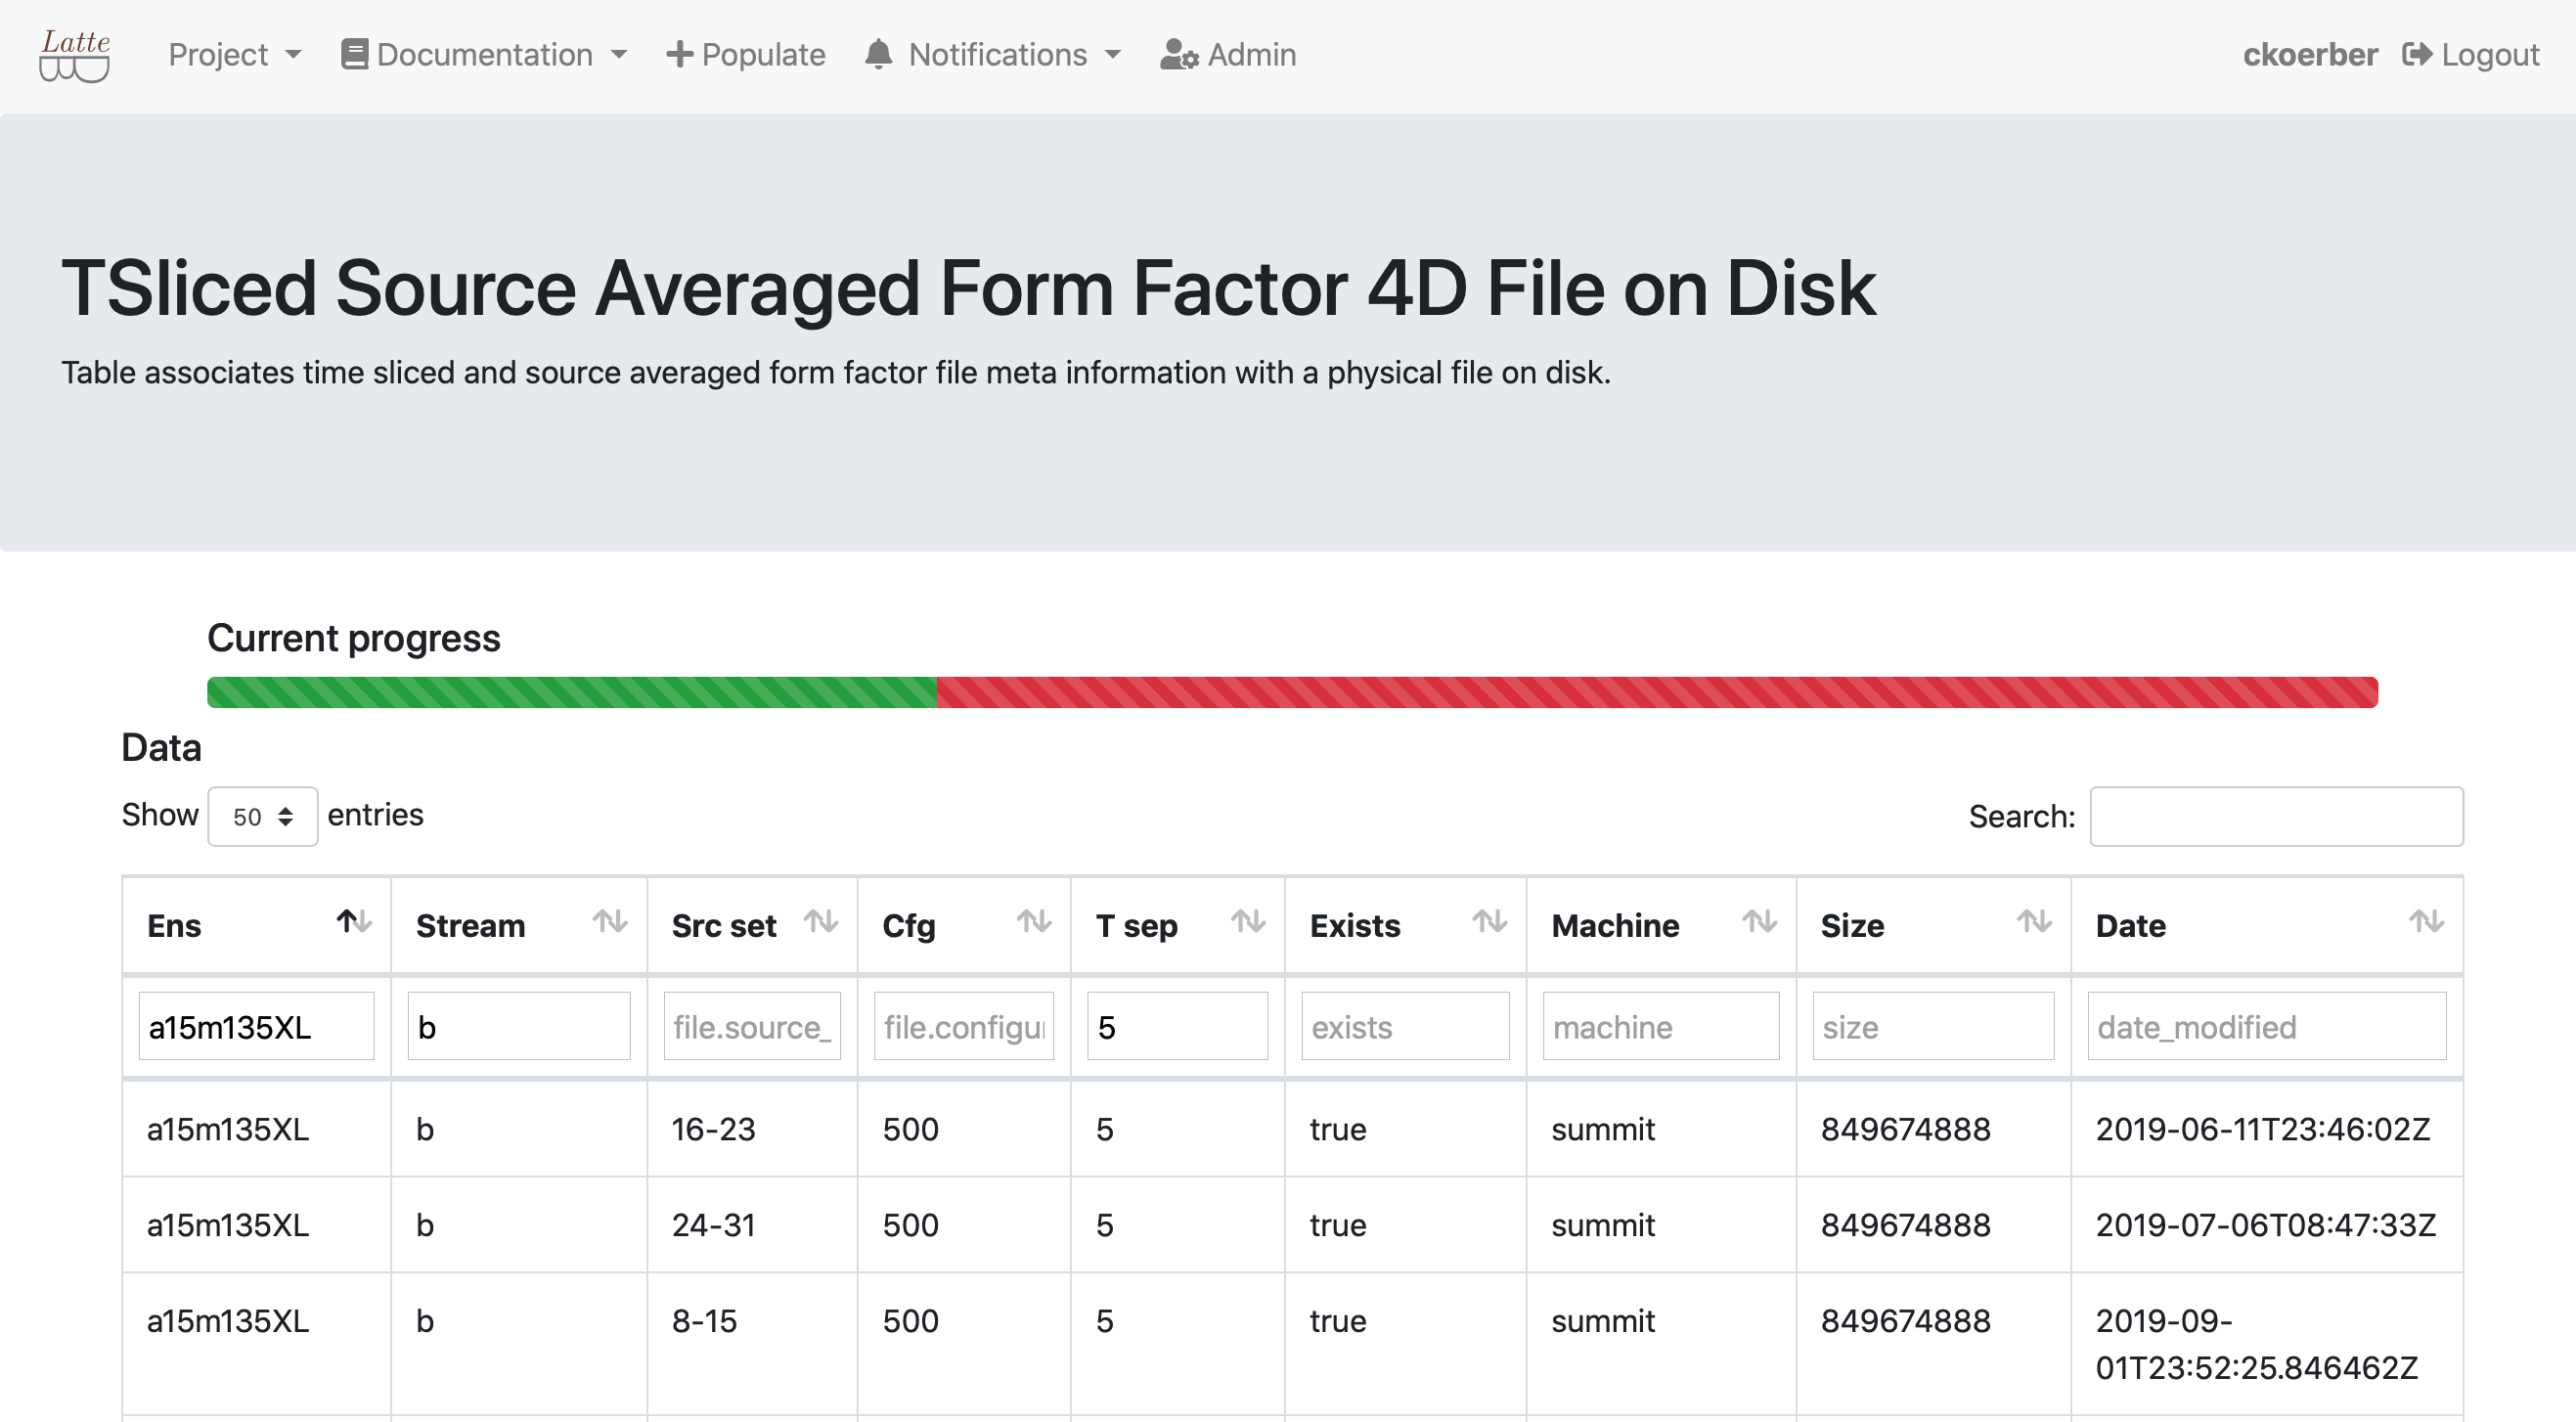
\includegraphics{lattedb-example.png}
\caption{Example table view of file status with column specific filters
and dynamic progress bar.}
\end{figure}

More importantly, our production scripts interact with \texttt{LatteDB},
therefore even without the visualization, the scripts will only generate
work that \texttt{LatteDB} records as missing. This interaction with
\texttt{LatteDB} significantly reduces the amount of human time required
to manage the computations. We are actively constructing routines to
also store the final data files to tape, the status of which is stored
in a related \texttt{LatteDB} table. Thus, the user can query the
database instead of the file system for the existence of data files,
significantly reducing the load on the file system as well.
Examples of interacting with \texttt{LatteDB} can be found in
our management repository for these INCITE projects
\url{https://github.com/callat-qcd/nucleon_elastic_FF}.
The scripts for interacting with \texttt{LatteDB} are in the \texttt{scripts} folder and contain \texttt{lattedb} in the name.
Other examples can be found in the \texttt{notebooks} folder in
\texttt{LatteDB}. These scripts will be updated regularly to encompass
more and more utilities from \texttt{EspressoDB} providing a complete
working example.

Other features that can be implemented is the storing of the data files
in \texttt{LatteDB} as well as storing the analysis of the data files.
This allows for communal data analysis within a collaboration with a
centralized location for results, making it easier to combine results
from different members and reduce redundant work. Depending upon the
success and popularity of \texttt{EspressoDB}, it may be worth exploring
whether OLCF (or other LCF) would be willing to allow users to host
databases locally on the machines such that the compute nodes could
interact with the database allowing users to minimize the number of
small input files that are typically written to the file system as well.
In our case, each separate task requires an input file and typically
generates two or three small output files, rapidly polluting the file
system with millions of small files. \texttt{EspressoDB} will minimally
allow users to \emph{clean up} these small files and store the relevant
log and output information in the database.




\end{document}
